\newpage
\section{Results} \label{results}
This chapter is dedicated to the presentation and description of the test results. Together with the literature review this chapter will lay a foundation for the later discussion on the aim of this research. The following tables contain the different results of all test runs. As described in the previous chapter, test one and test two were carried out for both JavaScript and WASM with three different inputs of ten test runs each. Test three was also performed for both JavaScript and WASM. In contrast to tests one and two, the entire test was carried out with five different inputs and only once with five test runs.
All result tables have an identical structure. The header row shows the number of test runs and the header column shows the respective input, categorised by JavaScript and WASM. In addition, there is an average and the standard deviation for each row. The first two tests were initially carried out with an input of 1,000,000. It was noticed that the results are not meaningful. Therefore the inputs have been gradually increased to reach an optimum in terms of runtime and credibility of the results. This approach identified 100,000,000 as the optimal input size for the first two tests. The same approach was used for the third test with a starting input of 100. This established optimum input for the third test at 30,000. From here on, we will therefore only deal with the results of the optimum input value.
\begin{figure}[H]
    \centering
    \caption[]{Table for results of test 1}
	\label{fig:tableTest1}
    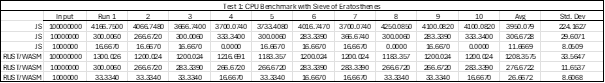
\includegraphics[width=1\textwidth]{table_test_1.png}
\end{figure}
In the first test, the lowest value for the runtime of JavaScript is 3666.74 ms and the highest value is 4250.09 ms. The average value is 3950.08 ms and the standard deviation is 224.16. For WASM, the lowest value is 1183.36 ms and the highest value is 1300.03 ms. The average value is 1208.36 ms and the standard deviation is 33.56.
\begin{figure}[H]
    \centering
    \caption[]{This is our website}
	\label{fig:tableTest2}
    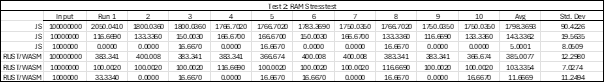
\includegraphics[width=1\textwidth]{table_test_2.png}
\end{figure}
In the second test, the lowest value for the runtime of JavaScript is 1750.04 ms and the highest value is 2050.04 ms. The average value is 1798.37 ms and the standard deviation is 90.42. For WASM, the lowest value is 366.67 ms and the highest value is 400.00 ms. The average value is 385.01 ms and the standard deviation is 12.30.
\begin{figure}[H]
    \centering
    \caption[]{This is our website}
	\label{fig:tableTest3}
    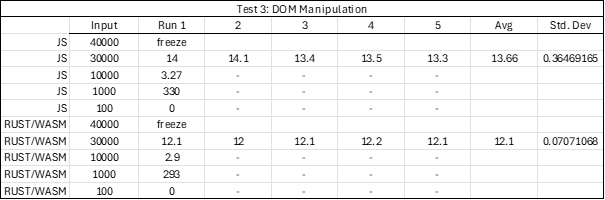
\includegraphics[width=1\textwidth]{table_test_3.png}
\end{figure}
In the last test, the lowest value for the runtime of JavaScript is 13.3 s and the highest value is 14.1 s. The average value is 1798.37 ms and the standard deviation is 90.42. The average value is 13.66 s and the standard deviation is 0.36. For WASM, the lowest value is 12.0 s and the highest value is 12.2 s. The average value is 12.1 s and the standard deviation is 0.07.